\section{Opnåede erfaringer}
\label{ch:OpXP}
\subsection{Generelt}
Gruppens fem medlemmer har været fordelt på fire forskellige projektgrupper i de tidligere projektforløb. Alle medlemmer er gået ligeværdigt ind i projektet med en positiv indstilling. Det har dog vist sig at være en større opgave at skabe en ny gruppe, end gruppen umiddelbart havde forestillet sig - og gruppen har ikke været sig denne opgave bevidst nok. Det har været en opgave for gruppen at forsøge at tage det bedste fra hver af de fire tidligere gruppe og stykke sammen til en ny. På trods af at grupperne har gennemgået samme undervisning er det meget forskelligt hvordan de forskellige grupper har anskuet processen, rollefordelinger, metoder og faser. Der har også skullet afstemmes forventninger og gruppen har ligeledes haft brug for at se hinanden an fagligt. Det har således været sværere i projekts opstartsperiode at vurdere hvor stor en opgave gruppen har kunnet påtage sig. Travlheden i slutningen af implementeringsfasen kan muligvis være en konsekvens heraf.
\\

\textbf{Faseforståelse}\\
I slutningen af projektforløbet blev forståelsen af systemarkitekturens formål væsentlig forbedret. Vi ved ikke hvor langt vi er kommet men det er vores helt klare opfattelse at vi er kommet et langt stykke videre i forståelsen af systemarkitekturen. Den forståelse vi har nu ligger på et markant højere niveau end den forståelse nogen af de fire grupper havde i de tidligere projektforløb. Det er ikke blot systemarkitekturen men hele samspillet imellem hovedfaserne. Formålet med kravspecifikationen set fra kundens synspunkt, overgangen derfra til systemarkitekturen ved hjælp af applikations og domænemodeller. Herfra virker springet til design og implementeringsfasen som en leg. \\
Den overgang var på ingen måde en leg for gruppen. Derimod blev faserne arkitektur og design nærmest sprunget let og elegant over. Dette har bidraget til en implementeringsfase hvor modulerne godt nok er blevet implementeret - og hvor de virker efter hensigten når man ser på dem individuelt. Problemerne begynder dog at opstå når modulerne begynder at blive sat sammen. Her bliver det tydeligt at arkitekturen og designdelen ikke har været tilfredsstillende nok. Spørgsmål som "Hvordan gør dit modul, når dette sker?" kan ikke blive besvaret i dokumentationen, men må stilles til personen der har implementeret modulet. I slutfasen er use cases og systemarkitekturen blevet kigget igennem en ekstra gang og der er blevet kigget nærmere på applikationsmodeller og domænemodeller. Gruppen forsøgte også det tidligere i forløbet, men forståelsen var ikke nok på plads, og motivationen var ikke stor nok til at det blev forsøgt ihærdigt nok. Dette kan givetvis også skyldes den lidt manglende kommunikation i projektet hvor der blev arbejdet i fem forskellige lejre - se erfaringen "uddelegering af opgaver".\\
Det ligger dog givetvis også en pointe i at domæne og applikationsmodeller er nemmere at opbygge for et system, som man har et indgående kendskab til fordi det er blevet implementeret. De frustrationer vi oprindeligt havde ved applikationsmodeller og domænemodeller udskød vi nok angiveligt til vi sad i implementeringsfasen. Og så igen når vi sad i testfasen og skulle sætte modulerne sammen. Erfaringen må være at jo tidligere i forløbet vi tager tyren ved hornene, jo "billigere" er det i arbejdstid - eller sagt på en anden måde: Selvom opgaven ser stor ud, så bliver den kun større af at vente med den.\\


\textbf{Pointer og brainstorm}\\
Vi har implementeret for hurtigt\\
Vi er kommet til at hoppe fra teknologiundersøgelser til implementering - og dermed sprang vi implementerings og designfasen over.\\
Vi har ikke været motiveret for at arbejde med systemarkitekturen fordi vi ikke havde forståelsen for nødvendigheden af den. Vi spurgte os selv: "Hvad bidrager den med?". Vi vidste det ikke.\\
Vi har tidligere i de fire forskellige grupper kun svagt - eller helt undladt - at anvende domæne- og applikationsmodeller. Dette har skyldtes at processen har været tung og at der ikke har været en godbid i den anden ende - vi har ikke kunnet se frugten af arbejdet.\\
Da vi var i systemarkitekturfasen var vi allerede dybt opslugt af teknologiundersøgelser - undersøgelser som begyndte mere at ligne implementeringer. Derfor var incitamentet for at begynde at strukturere systemet lavt. Gruppen var så opslugt af implementeringen at de forsøg der blev gjort for at få hul på bylden blev overhørt. Efterhånden stoppede forsøgene og systemarkitekturen blev for den største del af gruppen henlagt. Dette kan skyldes formegentlig at for størstedelen af gruppens medlemmer har systemarkitekturen tidligere været et obligatorisk arbejde uden egentlig bidrag til processen - resultatet har simpelthen ikke været tydeligt nok.\\
Systemarkitekturen og designfasen har været i højere grad været en hæmsko end et redskab i processen. Det har været en obligatorisk dokumentationsdel som lagt hen af vejen er blevet lavet i slutningen af - eller i bedste fald ad hoc med - implementeringsfasen. Vi har ikke fået øjenene op for hvad systemarkitekturen har at bidrage med. Vi har ikke set fordelene ved den. Arbejdet har ikke været time-effecient nok. Og så har implementeringen bare været så meget mere interessant.\\

\textbf{Faseforståelse 2}\\
En stor del af læringen i forbindelse med et projekt ligger i processen. Det udviklede system er nærmere et middel end det er et mål for semesterprojektet. Målet hedder bedre faseforståelse. Forståelse for de faser en udviklingsproces indebærer. Hver fase har sit eget bidrag til processen. Igennem projektarbejdet stifter gruppen gentagne gange bekendtskab med faserne. Hele uddannelsen er en iterativ proces med ét mål: En god forståelse af udviklingsprocessen af et system.\\
For hver af gruppens medlemmer har der tidligere været en eller flere åbenbaringer i løbet af et semesterprojekt. Et tidspunkt hvor en fordelen ved at anvende en given metode går op for personen og bliver soleklar. Åbenbaringer giver en fantastisk følelse af at gennembryde en mur, at have gjort et fremskridt. Dette kan godt ske flere gange for samme metode. Dette behøver ikke at betyde at de tidligere åbenbaringer har været forkerte, men blot at man er kommet et niveau højere op i sin forståelse. Hver åbenbaring er således noget positivt.\\
For dette semesterprojekt har den helt store åbenbaring indtruffet sent - om end med meget stor kraft.
Åbenbaringen er to-delt, men er faldet i samme tidsrum, da de har en tæt kobling.\\
Domæne- og applikationsmodeller i systemarkitekturen har tidligeret været et mystisk fænomen for en stor del af gruppen. Det har ikke været tydeligt hvad formålet - og frugten - var med det arbejde der blev lagt i modellerne. De har været frustrerende at udarbejde og det har ikke været klart hvordan de dernæst skulle anvendes. Således er incitamentet for at lave dem faldet, og flere af de tidligere grupper har slet og ret ikke har dem med i deres arkitektur. Omend det kan have været en korrekt beslutning  at udelade dem i tidligere projekter har gruppen sent i dette projekt set hvilket fantastisk redskab det kunne have været tidligere i processen. Da gruppen naturligt stødte på applikations- og domænemodeller i systemarkitekturfasen blev forsøget på at starte udarbejdelsen mødt med lavt engagement fra gruppen. Dette gjorde sig faktisk gældende for hele systemarkitekturfasen, omend i særlig høj grad for disse to modeltyper.\\
De to modeltyper blev så senere taget op igen af projektvejlederen. Der blev samtidig stilt nogle relevante spørgsmål til kravspecifikationen. Derpå blev kravspecifikationen og systemarkitekturen påny taget op ad gruppen. Her indtraf åbenbaringen en lørdag eftermiddag og kan sammenfattes til disse to sætninger:\\
Kravspecifikationen skal ses ud fra kundens perspektiv og dermed indeholde de informationer der for kunden er relevante.
Domæne og applikationsmodeller er nøddeknækkeren til kravspecifikationen - et redskab der transformerer use cases til konceptuelle klasser der kan laves sekvensdiagrammer ud fra (Sekvensdiagrammer er top nice!)\\

Denne nyfundne forståelse medførte en revision af kravspecifikation og systemarkitekturen med en stor mængde rettelser til følge. Det blev hurtigt tydeligt hvordan dette redskab, hvis anvendt korrekt, kunne have gjort at gruppen havde undgået en del frustration, problemer og smårettelser i slutningen af udviklingsfasen - især i testfasen. Enhedstesten gik fint. Integrationstesten gik dog ikke lige så gnidningsfrit:
I implementeringsfasen opstod behovet for at aftale hvordan specifikke situationer tackles ofte og en aftale blev derfor lavet mundtligt som følge af manglen på et fælles referencepunkt i en stringent og udførlig systemarkitektur. Problemerne det medførte blev først opdaget i integrationstesten hvor adskillige småændringer var nødvendige for at modulerne kunne kommunikere tilfredsstillende. I testforløbet blev behovet for en række mindre ændringer synliggjort. Dette er formegentlig naturligt for et testforløbet, men det er gruppens klare formodning at en del af disse valg burde have været truffet tidligere i processen - eksempelvis i arkitekturen.\\

\textbf{Rammer for projektet}\\
Omend det kan være rart at have frie tøjler er det gruppens erfaring at tøjlerne for dette projektforløb har været for frie. Enten har opgaven været for uinspirerende eller også har gruppen været for fantasiløs. Det var i hvert fald svært for gruppen at finde et projekt, der blev fundet både interessant nok samtidig med at faglige niveau var højt nok.\\

\textbf{Uddelegering af opgaver}\\
Gruppen har fra start ville uddelegere opgaver og ansvar for at lette arbejdsprocessen. Systemet blev derfor opdelt i moduler med en ansvarlig tilknyttet. Modulerne blev uddelt efter interesse. Dette har været en rigtig god løsning for flere af gruppens medlemmer tidligere, men i dette forløb har det vist sig også at være en hæmsko. Det fælles projektarbejde blev hurtigt fem personer, der sad med hvert deres lille område af projektet. Den interne kommunikation udeblev, og sparringen blev mangelfuld på grund af manglende indsigt i hvad de resterende gruppemedlemmer lavede.\\

\textbf{Programmering}\\
Gruppen har i dette projekt bestået af 5 elektronik ingeniørstuderende. Dette har skabt nogle problemer med hensyn til programmeringsdele af projektet. Gruppen har dog været god til at søge hjælp til problematiske opgaver, hvilket har gjort at programmeringstunge moduler er blevet implementeret korrekt.\\

\textbf{Vigtigheden af en struktureret faseinddeling}\\
For de fleste moduler i systemet startede implementeringen ret tidligt. Dette skyldtes for det første at det er denne fase gruppens medlemmer finder mest interessant, men ligeledes at det indledende arbejde gav blod på tanden til at afprøve de problemløsninger der langsomt begyndte at forme sig. Således gik en del af teknologiundersøgelsen ud på at afprøve nogle af disse problemløsninger, og før man har set sig om har man sprunget både systemarkitektur og designfasen over. Dette har for mere end et modul ført til en omskrivning af hele programmet op til flere gange. Disse omskrivninger har bl.a. været som følge af dårlig strukturet kode som følge af mange ændringer. Dette medførte hurtigt en besværliggørelse af læsningen af, og det videre arbejde med, koden. Tillige har det været svært at arbejde med koden i et tilfredsstillende tempo, da programmet ikke har været udformet og designet tilstrækkeligt inden implementeringsfasen. Erfaringen må være at et program hurtigt bliver større end hvad der kan overskues i hovedet af projektgruppens medlemmer på deres nuværende niveau. Vigtigheden af at faserne bliver benyttet er dermed større end først antaget.\\

\subsection{Rettidig test}
\subsection{Udvikling af hældningssensor}
Vi har startede med at udvikle på en prototype af en libellesensor vist på \textit{Figur~\ref{fig:libelle}}.
\begin{figure}[hbpt]
\centering
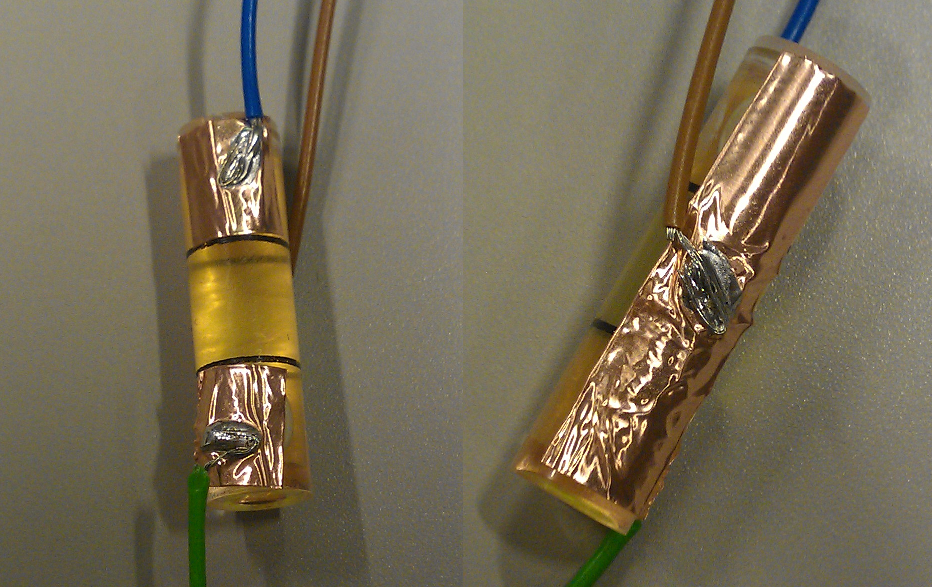
\includegraphics[width=0.5\textwidth]{billeder/libellesensor1}
\caption{henning}
\label{fig:libelle}
\end{figure}
Vi kom frem til at den har en capacitet på omkring $1*10^{-15}[F]$. Det gør det praktisk umuligt at anvende da vores filter så har en alt for stor cutoff frekvens liggende over 3.0 MHz. Den høje frekvens giver en stor selvinduktion i vores ledning. Samtidig kan vi ikke lave sinus med denne frekvens med PSoC'en. Dette gjorde at vi måtte finde en anden løsning.\\
Næste prototype bestod af et potmeter og et pendul. Dog havde potmeteret en for stor friktionsmodstand, der gjorde det upræcist i forhold til vores krav.\\
Vi har gennem et tredje semestersfag fundet ud af at PSoC'en indeholder et accelerometer. Vi valgte så at lave en prototype med det. Dette viste sig at være en god løsning.

\subsection{Metoder}
Gruppen var opsatte på at have læst review på projektets dokumentation, men de adspurgte grupper havde ingen interesse i at lave review udvekslinger. Dette har ført til at dokumentationen blev gennemlæst på et senere tidspunkt af gruppens vejleder. Grundet udskydelsen havde gruppen set sig nødsaget til at forlænge tidsplanen for at opdatere og forbedre foreløbigt færdig dokumentation. Dette førte til at design og, i sidste ende, implementering blev udskudt, hvilket medfører et stort pres imod slutningen af projektforløbet.\\
Gruppens opdeling i udviklingsmetoden har været meget flydende. Selv om der har været en projektleder og scrummaster har det ikke været nødvendigt, da gruppen har arbejdet godt sammen og diskuteret udviklingsmetoden til fuldest. Der har i forløbet været en udskiftning i koordinatorposten, hvorefter rumkoordinering har forløbet godt.\\
Gruppen har fået en bedre forståelse for eventuelt kommunikation med en kunde gennem flere iterationer af kravspecifikation.

\subsection{Udvikling af afstandssensor}
Ultralydsafstandsmålingen blev valgt for at prøve noget ingen havde kendskab til i projektet. Man kunne have valgt at købe en færdiglavet enhed men det blev vurderet at dette ikke gav ret meget faglig erfaring. I e-lab havde de nogle rå tranducere og receivere liggende og der blev derfor valgt at forsøge med at udvikle en ultralydsafstandsmåler. Der blev i starten lavet en del teknologiundersøgelse inden for ultralyden og vi testede tranducere og receivere for at se hvordan de aggerede. Vi fandt at der var en del destruktive reflektioner og vi overvejede at fylde akustisk skum i toppen af tankene, men da det skum vi kunne finde var elektrisk ledende kunne vi ikke anvende det. Jeg kom frem til at et burst skulle sendes for at måle afstanden og en puls på 250$\mu$s blev valgt, hvilket svarer til 10 perioder. Receiverkredsen blev udviklet med viden fra MSE kurset fra sidste semester omkring mixere og operationsforstærkere. Den største erfaring opnået gennem dette forløb må være at man bare, som hovedregel, bare selv skal købe noget der passer til formålet og implementere dette i projektet. Dette giver mere plads til at lave et større system, simplere. Derudover gav det god erfaring i mixerelektronik og ultralydsteknologi, som er meget besværligt at arbejde med.

\subsection{Udvikling af Databasen}
